\documentclass{standalone}
\usepackage{tikz}
\usetikzlibrary{patterns, positioning}
\usepackage[sfdefault]{ClearSans} %% option 'sfdefault' activates Clear Sans as the default text font
\usepackage[T1]{fontenc}

\begin{document}
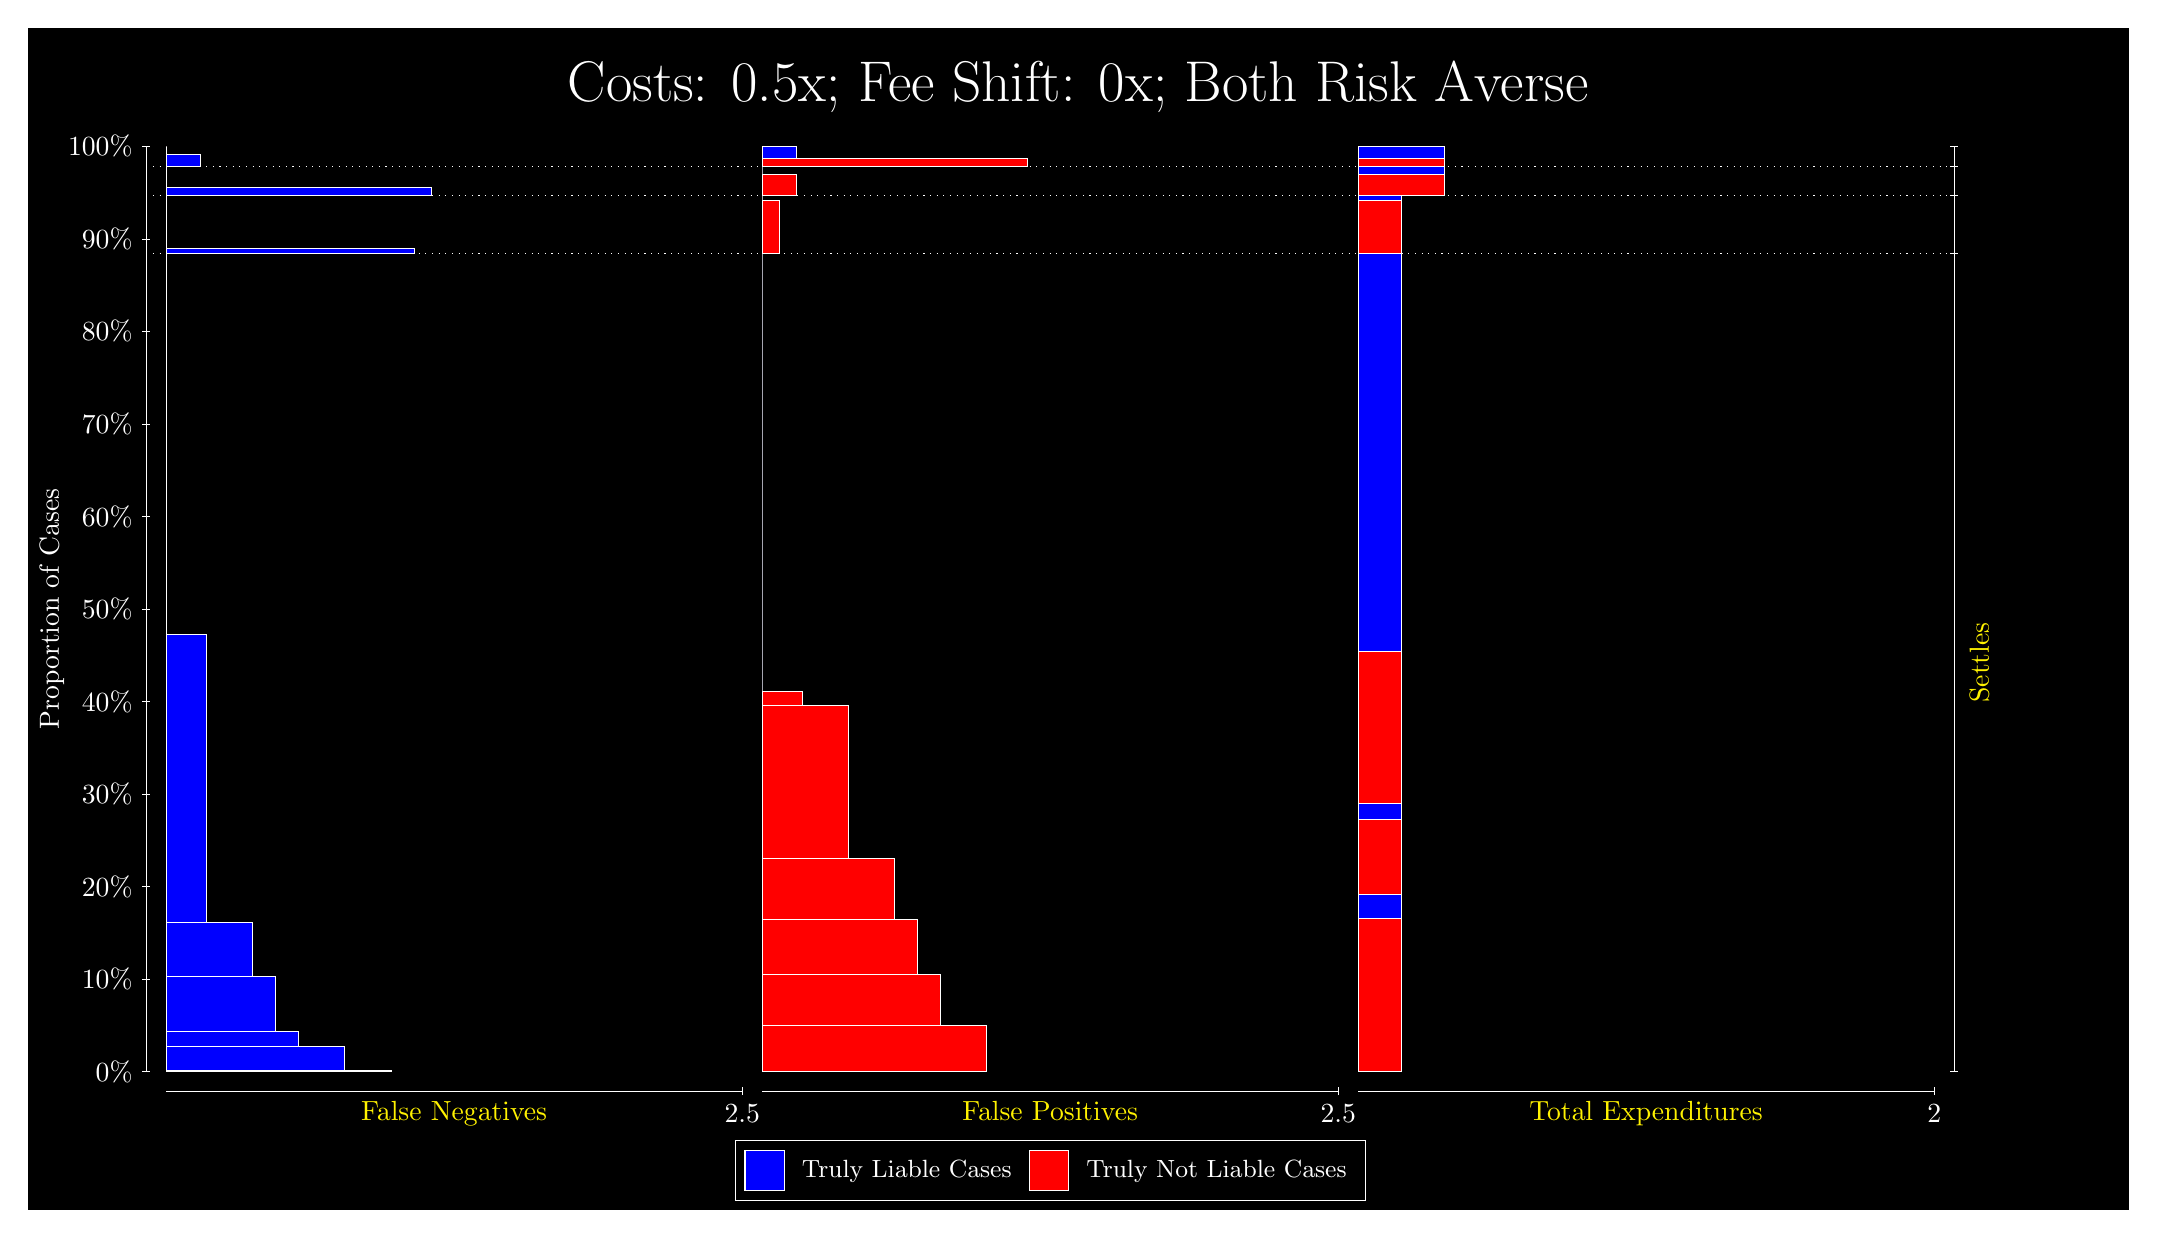
\begin{tikzpicture}
\draw[fill=black] (0,0) rectangle (26.667,15);
\draw[text=white] (0,13.5) rectangle (26.667,15) node[midway] {\huge Costs: 0.5x; Fee Shift: 0x; Both Risk Averse};
\draw[white, very thin] (1.5,1.75) -- (1.5,13.5);
\node[rotate=90, text=white, anchor=center] at (0.3, 7.625) {Proportion of Cases};
\draw[white, very thin] (1.45,1.75) -- (1.55,1.75);
\node[text=white, anchor=east] at (1.45, 1.75) {0\%};
\draw[white, very thin] (1.45,2.925) -- (1.55,2.925);
\node[text=white, anchor=east] at (1.45, 2.925) {10\%};
\draw[white, very thin] (1.45,4.1) -- (1.55,4.1);
\node[text=white, anchor=east] at (1.45, 4.1) {20\%};
\draw[white, very thin] (1.45,5.275) -- (1.55,5.275);
\node[text=white, anchor=east] at (1.45, 5.275) {30\%};
\draw[white, very thin] (1.45,6.45) -- (1.55,6.45);
\node[text=white, anchor=east] at (1.45, 6.45) {40\%};
\draw[white, very thin] (1.45,7.625) -- (1.55,7.625);
\node[text=white, anchor=east] at (1.45, 7.625) {50\%};
\draw[white, very thin] (1.45,8.8) -- (1.55,8.8);
\node[text=white, anchor=east] at (1.45, 8.8) {60\%};
\draw[white, very thin] (1.45,9.975) -- (1.55,9.975);
\node[text=white, anchor=east] at (1.45, 9.975) {70\%};
\draw[white, very thin] (1.45,11.15) -- (1.55,11.15);
\node[text=white, anchor=east] at (1.45, 11.15) {80\%};
\draw[white, very thin] (1.45,12.325) -- (1.55,12.325);
\node[text=white, anchor=east] at (1.45, 12.325) {90\%};
\draw[white, very thin] (1.45,13.5) -- (1.55,13.5);
\node[text=white, anchor=east] at (1.45, 13.5) {100\%};

\draw[white, very thin] (24.457,1.75) -- (24.457,13.5);
\draw[white, very thin] (24.407,1.75) -- (24.507,1.75);
\node[anchor=west] at (24.407, 1.75) {};
\draw[white, very thin] (24.407,12.139) -- (24.507,12.139);
\node[anchor=west] at (24.407, 12.139) {};
\draw[white, very thin] (24.407,12.877) -- (24.507,12.877);
\node[anchor=west] at (24.407, 12.877) {};
\draw[white, very thin] (24.407,13.246) -- (24.507,13.246);
\node[anchor=west] at (24.407, 13.246) {};
\draw[white, very thin] (24.407,13.5) -- (24.507,13.5);
\node[anchor=west] at (24.407, 13.5) {};

\draw[white, very thin, fill=blue] (1.75,1.75) rectangle (4.6044,1.7623);
\draw[white, very thin, fill=blue] (1.75,1.7623) rectangle (4.0188,2.0683);
\draw[white, very thin, fill=blue] (1.75,2.0683) rectangle (3.4333,2.255);
\draw[white, very thin, fill=blue] (1.75,2.255) rectangle (3.1406,2.9618);
\draw[white, very thin, fill=blue] (1.75,2.9618) rectangle (2.8478,3.6515);
\draw[white, very thin, fill=blue] (1.75,3.6515) rectangle (2.2623,7.307);
\draw[white, very thin, fill=red] (1.75,7.307) rectangle (1.75,12.139);
\draw[white, very thin, fill=blue] (1.75,12.139) rectangle (4.8971,12.202);
\draw[white, very thin, fill=red] (1.75,12.202) rectangle (1.75,12.877);
\draw[white, very thin, fill=blue] (1.75,12.877) rectangle (5.1167,12.977);
\draw[white, very thin, fill=red] (1.75,12.977) rectangle (1.75,13.246);
\draw[white, very thin, fill=blue] (1.75,13.246) rectangle (2.1891,13.401);
\draw[white, very thin, fill=red] (1.75,13.401) rectangle (1.75,13.5);
\draw[white, very thin, fill=red] (9.3189,1.75) rectangle (12.173,2.3354);
\draw[white, very thin, fill=red] (9.3189,2.3354) rectangle (11.588,2.9793);
\draw[white, very thin, fill=red] (9.3189,2.9793) rectangle (11.295,3.6861);
\draw[white, very thin, fill=red] (9.3189,3.6861) rectangle (11.002,4.4546);
\draw[white, very thin, fill=red] (9.3189,4.4546) rectangle (10.417,6.405);
\draw[white, very thin, fill=red] (9.3189,6.405) rectangle (9.8312,6.5819);
\draw[white, very thin, fill=blue] (9.3189,6.5819) rectangle (9.3189,12.139);
\draw[white, very thin, fill=red] (9.3189,12.139) rectangle (9.5384,12.814);
\draw[white, very thin, fill=blue] (9.3189,12.814) rectangle (9.3189,12.877);
\draw[white, very thin, fill=red] (9.3189,12.877) rectangle (9.758,13.147);
\draw[white, very thin, fill=blue] (9.3189,13.147) rectangle (9.3189,13.246);
\draw[white, very thin, fill=red] (9.3189,13.246) rectangle (12.686,13.345);
\draw[white, very thin, fill=blue] (9.3189,13.345) rectangle (9.758,13.5);
\draw[white, very thin, fill=red] (16.888,1.75) rectangle (17.437,3.7005);
\draw[white, very thin, fill=blue] (16.888,3.7005) rectangle (17.437,4.0065);
\draw[white, very thin, fill=red] (16.888,4.0065) rectangle (17.437,4.9518);
\draw[white, very thin, fill=blue] (16.888,4.9518) rectangle (17.437,5.1507);
\draw[white, very thin, fill=red] (16.888,5.1507) rectangle (17.437,7.0869);
\draw[white, very thin, fill=blue] (16.888,7.0869) rectangle (17.437,12.139);
\draw[white, very thin, fill=red] (16.888,12.139) rectangle (17.437,12.814);
\draw[white, very thin, fill=blue] (16.888,12.814) rectangle (17.437,12.877);
\draw[white, very thin, fill=red] (16.888,12.877) rectangle (17.986,13.147);
\draw[white, very thin, fill=blue] (16.888,13.147) rectangle (17.986,13.246);
\draw[white, very thin, fill=red] (16.888,13.246) rectangle (17.986,13.345);
\draw[white, very thin, fill=blue] (16.888,13.345) rectangle (17.986,13.5);
\draw[white, dotted] (1.5,12.139) -- (24.457,12.139);
\draw[white, dotted] (1.5,12.877) -- (24.457,12.877);
\draw[white, dotted] (1.5,13.246) -- (24.457,13.246);
\draw[white, very thin] (1.75,1.5) -- (9.0689,1.5);
\node[text=yellow, anchor=north] at (5.4094, 1.5) {False Negatives};
\draw[white, very thin] (9.0689,1.45) -- (9.0689,1.55);
\node[text=white, anchor=north] at (9.0689, 1.45) {2.5};

\draw[white, very thin] (9.3189,1.5) -- (16.638,1.5);
\node[text=yellow, anchor=north] at (12.978, 1.5) {False Positives};
\draw[white, very thin] (16.638,1.45) -- (16.638,1.55);
\node[text=white, anchor=north] at (16.638, 1.45) {2.5};

\draw[white, very thin] (16.888,1.5) -- (24.207,1.5);
\node[text=yellow, anchor=north] at (20.547, 1.5) {Total Expenditures};
\draw[white, very thin] (24.207,1.45) -- (24.207,1.55);
\node[text=white, anchor=north] at (24.207, 1.45) {2};

\node[text=yellow, centered, rotate=90] at (24.777, 6.9444) {Settles};




\draw (12.978300999999998,1.5) node[draw=none] (baseCoordinate) {};
\begin{scope}[align=center]
        \matrix[scale=0.5, draw=white, below=0.5cm of baseCoordinate, nodes={draw}, column sep=0.1cm]{
            \node[rectangle, draw, minimum width=0.5cm, minimum height=0.5cm, fill=blue] {}; &
            \node[draw=none, font=\small, text=white] (B) {Truly Liable Cases}; &
            \node[rectangle, draw, minimum width=0.5cm, minimum height=0.5cm, fill=red] {}; &
            \node[draw=none, font=\small, text=white] (B) {Truly Not Liable Cases}; \\
            };
\end{scope}

\end{tikzpicture}
\end{document}